
\documentclass[10pt,letterpaper]{article}
\usepackage[top=0.85in,left=2.75in,footskip=0.75in]{geometry}

% amsmath and amssymb packages, useful for mathematical formulas and symbols
\usepackage{amsmath,amssymb}

% Use adjustwidth environment to exceed column width (see example table in text)
\usepackage{changepage}

% textcomp package and marvosym package for additional characters
\usepackage{textcomp,marvosym}

% cite package, to clean up citations in the main text. Do not remove.
\usepackage{cite}

% Use nameref to cite supporting information files (see Supporting Information section for more info)
\usepackage{nameref,hyperref}

% line numbers
\usepackage[right]{lineno}

% ligatures disabled
\usepackage[nopatch=eqnum]{microtype}
\DisableLigatures[f]{encoding = *, family = * }

% color can be used to apply background shading to table cells only
%\usepackage[table]{xcolor}

% array package and thick rules for tables
\usepackage{array}

% create "+" rule type for thick vertical lines
\newcolumntype{+}{!{\vrule width 2pt}}

% create \thickcline for thick horizontal lines of variable length
\newlength\savedwidth
\newcommand\thickcline[1]{%
  \noalign{\global\savedwidth\arrayrulewidth\global\arrayrulewidth 2pt}%
  \cline{#1}%
  \noalign{\vskip\arrayrulewidth}%
  \noalign{\global\arrayrulewidth\savedwidth}%
}

% \thickhline command for thick horizontal lines that span the table
\newcommand\thickhline{\noalign{\global\savedwidth\arrayrulewidth\global\arrayrulewidth 2pt}%
\hline
\noalign{\global\arrayrulewidth\savedwidth}}


% Remove comment for double spacing
%\usepackage{setspace} 
%\doublespacing

% Text layout
\raggedright
\setlength{\parindent}{0.5cm}
\textwidth 5.25in 
\textheight 8.75in

% Bold the 'Fig #' in the caption and separate it from the title/caption with a period
% Captions will be left justified
\usepackage[aboveskip=1pt,labelfont=bf,labelsep=period,justification=raggedright,singlelinecheck=off]{caption}
\renewcommand{\figurename}{Fig}

% Use the PLoS provided BiBTeX style
\bibliographystyle{plos2015}

% Remove brackets from numbering in List of References
\makeatletter
\renewcommand{\@biblabel}[1]{\quad#1.}
\makeatother



% Header and Footer with logo
\usepackage{lastpage,fancyhdr,graphicx}
\usepackage{epstopdf}
\usepackage{lmodern}
%\pagestyle{myheadings}
\pagestyle{fancy}
\fancyhf{}
%\setlength{\headheight}{27.023pt}
%\lhead{\includegraphics[width=2.0in]{PLOS-submission.eps}}
\rfoot{\thepage/\pageref{LastPage}}
\renewcommand{\headrulewidth}{0pt}
\renewcommand{\footrule}{\hrule height 2pt \vspace{2mm}}
\fancyheadoffset[L]{2.25in}
\fancyfootoffset[L]{2.25in}
\lfoot{\today}

%% Include all macros below

\newcommand{\lorem}{{\bf LOREM}}
\newcommand{\ipsum}{{\bf IPSUM}}

%% END MACROS SECTION

%% personal packages and macro
%%% packages
\usepackage[utf8]{inputenc}        % allow utf-8 input
\usepackage[T1]{fontenc}           % use 8-bit T1 fonts
\usepackage[dvipsnames, table]{xcolor}
\usepackage{tabularx}
\usepackage{multirow}
\usepackage{pifont}
\usepackage{csvsimple}
\usepackage[font={small},textfont={it},labelfont={bf}]{caption}
\usepackage{subcaption}
\usepackage{graphicx}
\usepackage{url}                   % simple URL typesetting
\usepackage{booktabs}              % professional-quality tables
\usepackage{makecell}
\usepackage{amsfonts}              % blackboard math symbols
\usepackage{amsmath}
\usepackage{nicefrac}              % compact symbols for 1/2, etc.
\usepackage{microtype}             % microtypography
\usepackage{enumitem}
\usepackage[export]{adjustbox}


%not compatible with cite package
%\usepackage[natbib=true,style=nature,maxnames=999,maxcitenames=2,backend=biber]{biblatex}
%\addbibresource{references.bib}

%%% macros
\DeclareMathOperator*{\argmin}{arg\,min}
\newcommand{\indep}{\perp \!\!\! \perp}
\newtheorem{assumption}{Assumption}

\definecolor{dark_blue}{rgb}{0,0,.65}
\definecolor{dark_green}{rgb}{0,.5,.15}

\hypersetup{pdftex,  % needed for pdflatex
  breaklinks=true,  % so long urls are correctly broken across lines
  colorlinks=true,
  linkcolor=dark_blue,
  citecolor=dark_green,
}
\colorlet{P}{ForestGreen}
\colorlet{I}{MidnightBlue}
\colorlet{C}{YellowOrange}
\colorlet{O}{DarkOrchid}
\colorlet{T}{Gray}



\begin{document}
\vspace*{0.2in}

\section*{Supporting information}

\paragraph*{S7 Appendix}
\label{apd:hte}
{\bf Details on treatment heterogeneity analysis.}

\textbf{Detailed estimation procedure}

The estimation of heterogeneous effect based on Double Machine Learning adds
another step after the computation, regressing the residuals of the outcome
nuisance $\tilde{Y} - \mu(X)$ against the residuals of the treatment nuisance
$\tilde{A} = A - e(X)$ with the heterogeneity features $X_{CATE}$. Noting the
final CATE model $\theta$, Double ML solves:

$$\argmin_{\theta} \mathbb E_n \big[(\tilde{Y} - \tau (X_CATE) \cdot \tilde{A})^2\big ]$$

Where $\tilde{Y} = Y - \hat m(X)$ and $\tilde{A} = A - \hat e(X)$

To avoid the over-fitting of this last regression model, we split the dataset of
the main analysis into a train set (size=0.8) where the causal estimator and the final
model are learned, and a test set (size=0.2) on which we report the predicted Conditional Average
Treatment Effects.

\textbf{Known heterogeneity of treatment for the emulated trial}\label{apd:cate_literature}

\cite{caironi2014albumin} observed statistical differences in the post-hoc
subgroup analysis between patient with and without septic shock at inclusion.
They found increasing treatment effect measured as relative risk for patients
with septic shock (RR=0.87; 95\% CI, 0.77 to 0.99 vs 1.13;95\% CI, 0.92 to 1.39).

\cite{safe2007saline} conducted a post-hoc subgroup analysis of patients with or
without brain injury --defined as Glasgow Coma Scale between 3 to 8--. The
initial population was patients with traumatic brain injury (defined as history
or evidence on A CT scan of head trauma, and a GCS score <= 13). They found
higher mortality rate at 24 months in the albumin group for patients with severe
head injuries.

\cite{zhou2021early} conducted a subgroup analysis on age (<60 vs >60), septic
shock and sex. They conclude for increasing treatment effect measured as
Restricted Mean Survival Time for Sepsis vs septic shock (3.47 vs. 2.58), for
age >=60 (3.75 vs 2.44), for Male (3.4 vs 2.69). None of these differences were
statistically significant.

\textbf{Vibration analysis}\label{apd:cate_results}

The choice of the final model for the CATE estimation should also be informed
by statistical and clinical rationals. Fig
\ref{apd:fig:albumin_for_sepsis:cate_boxplot_forest} shows the distribution of
the individual effects of a final random forest estimator, yielding CATE
estimates that are not consistent with the main ATE analysis. Fig
\ref{apd:fig:albumin_for_sepsis:cate_age_forest_failure} shows that the choice
of this final model imposes an inductive bias on the form of the heterogeneity
and different sources of noise depending of the nature of the model. A random
forest is noisier than a linear model. Fig
\ref{apd:fig:albumin_for_sepsis:cate_age_forest_failure} shows the difference
of modelization on the subpopulation of non-white male patients without septic
shock. One can see that the decreasing linear trend is reflected by the
random forest model only for patients aged between 55 and 80.

\begin{figure}[h!]
    \centering
    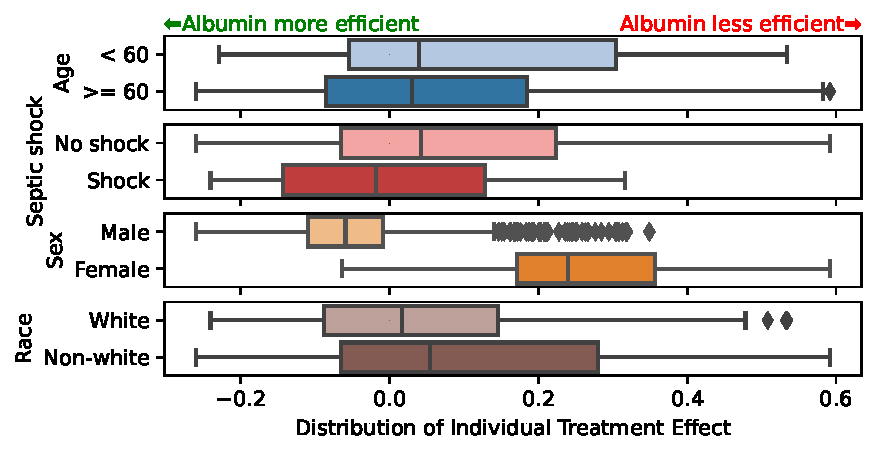
\includegraphics[width=0.8\linewidth]{img_supp_final/boxplot_est__DML__nuisances__Forests__final_RF.pdf}
    \caption{{\bf Values of Conditional Average Treatment effects on sex, age,
                race and pre-treatment septic shock estimated with a final forest
                estimator.}\\The CATE are positive for each subgroups, which is not
        consistent with the null treatment effect obtained in the main analysis.
        The boxes contain between the 25th and 75th percentiles of the CATE
        distributions with the median indicated by a vertical line. The whiskers
        extends to 1.5 the inter-quartile range of the
        distribution.}\label{apd:fig:albumin_for_sepsis:cate_boxplot_forest}
\end{figure}

\begin{figure}[h!]
    \centering
    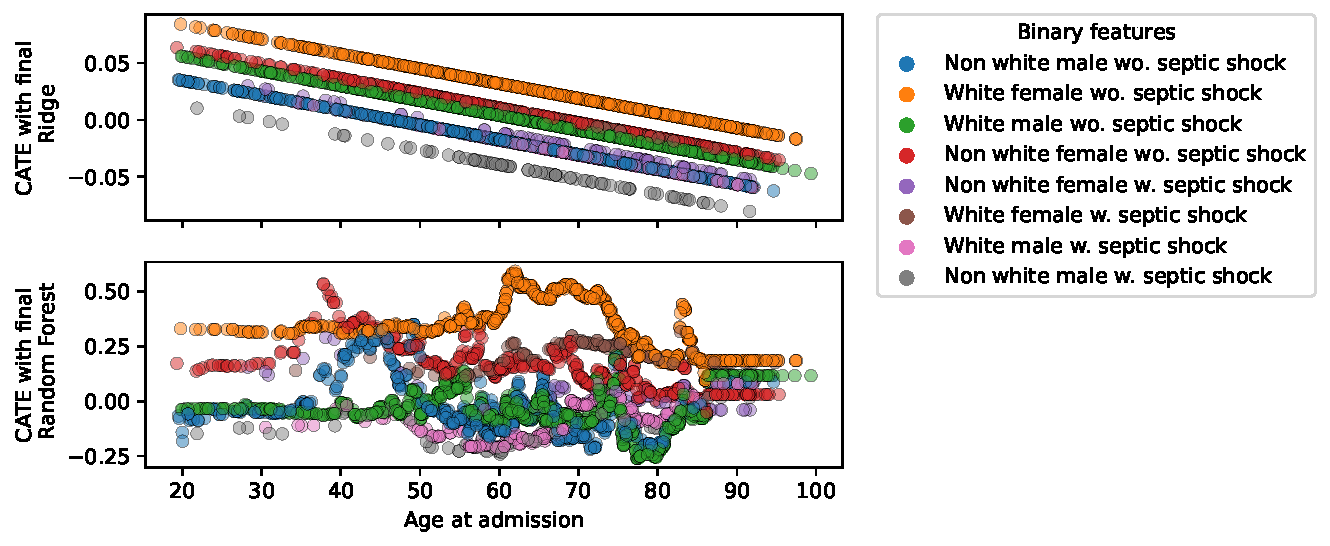
\includegraphics[width=\linewidth]{img_supp_final/cate_all_category_random_forest.pdf}
    \caption{{\bf Values of Conditional Average Treatment effects on sex, age,
                race and pre-treatment septic shock plotted for different ages.}\\On the top
        the final estimator is a linear model; on the bottom, it is a random
        forest. The forest-based CATE displays more noisy trends than the
        linear-based CATE. This suggest that the flexibility of the random forest
        might be underfitting the data.}\label{apd:fig:albumin_for_sepsis:cate_age_forest_failure}
\end{figure}

\clearpage
\begin{figure}[h!]
    \centering
    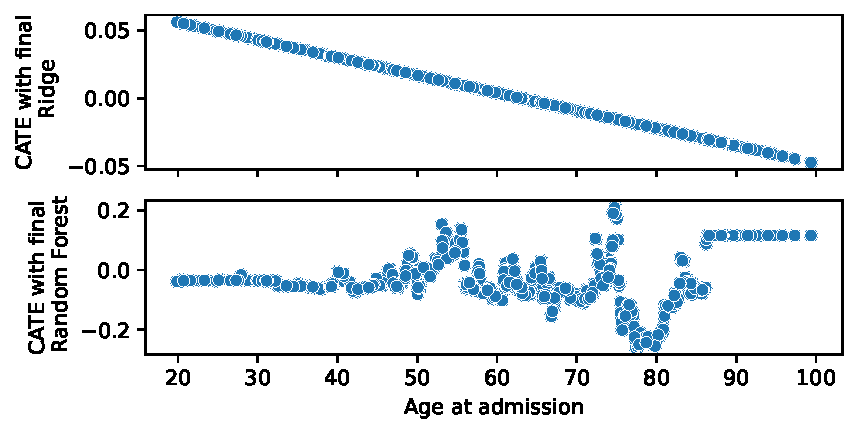
\includegraphics[width=\linewidth]{img_supp_final/cate_shock_random_forest.pdf}
    \caption{{\bf Values of Conditional Average Treatment effects on age, for the subpopulation of white male patients without septic shock.}\\ It is a subset of Fig \ref{apd:fig:albumin_for_sepsis:cate_age_forest_failure}. Contrary to
        the ridge regression (on top) inducing a nicely interpretable trend, using
        random forests as the final estimator failed to recover CATE on ages: the
        predicted estimates do not exhibit any trend and display inconsistently
        large effect sizes, suggesting data underfitting.
    }\label{apd:fig:albumin_for_sepsis:cate_failure}
\end{figure}


\bibliography{references}


\end{document}
